\Testart{Skript}
\Klasse{09}
\Fach{Informatik}
\Lehrer{Valentin Herrmann}
\Titel{Tabellenkalkulation}

    
%\large

\renewcommand{\Content}{

\input{_Aufgaben/A00_BYCSDrive}

\input{_Aufgaben/A01_ExcelWerbung}

\input{_Hefteintraege/H01_TabKalk}

\input{_Hefteintraege/H02_Formeln}

\input{_Aufgaben/A02_ExcelWerbung_Formeln}

\input{_Hefteintraege/H03_Zellbezug}

\Aufgabe[15]{Formeln mit Diagrammen darstellen}
{
Diagramme wie im ersten Hefteintrag, die Eingabe, Verarbeitung und Ausgabe darstellen, nennt man Datenflussdiagramm.
\begin{itemize}
    \item Zeichne für eine Wachstumsberechnung und eine Summe aus deiner Tabelle je ein Datenflussdiagramm.
    \item Überlege dabei: Wie stellst du die Daten dar und wieso?\\Zum Beispiel als konkreten Wert, als Zelladresse, als Beschreibung, ... ?
\end{itemize}
\doppelseite{0.48}{0.48}{t}{
    \ifloesung
        \LoesungTikz{
            \node[dfddata, text width=2.2cm, minimum width=3cm, minimum height=1cm] (golf) {Umsatz Golf Q2};
            \node[dfddata, text width=2.5cm, minimum width=3cm, minimum height=1cm, right=0.5cm of golf] (fakt) {Wachstums-faktor};

            \node[oval, text width=2.2cm, minimum width=3.5cm, minimum height=1.2cm, below=0.8cm of $(golf)!0.5!(fakt)$] (stern) {PRODUKT oder *};
            
            \node[dfddata, minimum width=3cm, minimum height=1cm, below=1cm of stern] (gq3) {Umsatz Golf Q3};
            
            \draw[arrow] (golf) -- (stern);
            \draw[arrow] (fakt) -- (stern);
            \draw[arrow] (stern) -- (gq3);
        }
    \else
        \begin{tikzpicture}[
            oval/.style={ellipse, draw, thick, minimum width=3.5cm, minimum height=1.2cm, align=center}
        ]
            \node[dfddata, minimum width=3cm, minimum height=1cm] (golf) {};
            \node[dfddata, minimum width=3cm, minimum height=1cm, right=0.5cm of golf] (fakt) {};
            \node[oval, below=0.8cm of $(golf)!0.5!(fakt)$] (stern) {};
            \node[dfddata, minimum width=3cm, minimum height=1cm, below=1cm of stern] (gq3) {};
        \end{tikzpicture}
    \fi
}{
    \LoesungKaroTikz{
        \node[dfddata, text width=2cm] (gq2) {Umsatz Golf Q2};
        \node[dfddata, text width=2.1cm, right=0.3cm of gq2] (tq2) {Umsatz Tennis Q2};
        \node[dfddata, text width=2.1cm, right=0.3cm of tq2] (sq2) {Umsatz Safari Q2};

        \node[oval, text width=2.2cm, below=0.8cm of tq2] (summe) {SUMME (nicht + ! )};
        
        \node[dfddata, below=1cm of summe] (final) {Gesamtumsatz Q2};
        
        \draw[arrow] (gq2) -- (summe);
        \draw[arrow] (tq2) -- (summe);
        \draw[arrow] (sq2) -- (summe);
        \draw[arrow] (summe) -- (final);
    }{22}
}
}

\input{_Hefteintraege/H04_Abstraktionsebenen}

\Aufgabe[20]{Der Weg der Daten}{
    \begin{minipage}[t]{0.85\textwidth}
        \begin{enumerate}
            \item Öffnet im Browser Orinoco: \UrlAndCode{klassenkarte.de/oo/}
            \item Aus der linken Spalte benötigen wir die Elemente \emphColB{Eingabe, Funktion, Ausgabe und Datenfluss}.
            \item Wählt zwei verschiedene Formelfelder eurer Tabelle aus und erstellt ein Diagramm mit den genannten Elementen, das darstellt, welche Daten in die Berechnung einfließen, welche ausgegeben werden und was für eine Berechnung durchgeführt wird.
            \item Erstellt möglichst viele Diagramme auf verschiedenen Abstraktionsebenen.
        \end{enumerate}
        
        \vspace{0.2cm}
        \Loesung{
            Ein paar Beispiele für eine Zelle. Es gibt natürlich sehr viele Möglichkeiten.\\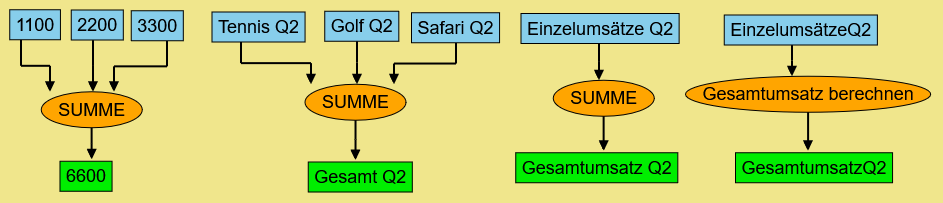
\includegraphics[width=\textwidth]{_Aufgaben/img/orinoo.png}
        }
    \end{minipage}
}


\input{_Hefteintraege/H05_DFD}

\input{_Hefteintraege/H06_Funktionen}

\input{_Aufgaben/A05_Getraenke}

\input{_Aufgaben/A06_DFDPuzzle}

\input{_Hefteintraege/H07_Verkettung}

\input{_Aufgaben/A07_FktModellierung}

\input{_Aufgaben/A08_FktModUmsetzen}

\input{_Hefteintraege/H08_WennDann}

\input{_Aufgaben/A09_Filter}

\input{_Hefteintraege/H09_Filter}

}